% eLife house format. Build with XeLaTeX (the class uses unicode-math):
%   xelatex main; bibtex main; xelatex main; xelatex main
% Every number traces to a CSV in ../data/ (see ../data/README.md).

\documentclass[9pt,lineno]{elife}

\graphicspath{{figures/}}

\title{Head-direction invariance, not information, determines whether a predictive cognitive
map folds under symmetry}

\author[1]{Manas Venkata Sai Ravulapalli}
\affil[1]{Ashoka University, Sonipat, India}
\corr{manasvenkatasai.ravulapalli\_ug2023@ashoka.edu.in}{MR}

\begin{document}
\maketitle

\begin{abstract}
\noindent
Predictive learning produces place-cell-like spatial codes in recurrent networks
\citep{levenstein2024}, but the arenas used to validate this are built so that every position
looks unique. Real arenas are symmetric, and symmetric landmarks make distinct positions
observationally identical. We train predictive recurrent networks in arenas with $C_1$, $C_2$
and $C_4$ rotational landmark symmetry and manipulate their head-direction input, comparing
conditions \emph{within} a single arena so the observation stream is held exactly fixed. The
decisive contrast holds information constant and varies only symmetry: two head-direction
encodings of exactly one bit each, one invariant under a $180^\circ$ rotation and one not. In
the $C_2$ arena the two separate completely in orbit-phase decoding ($p = 1.1\times10^{-5}$,
$n = 10$ networks per encoding); in the asymmetric arena they are indistinguishable
($p = 0.97$). Invariance, not information, folds the code, and the $C_4$ arena approaches the group-theoretic
$1/|G|$ ceiling. The effect requires prediction: a matched autoencoder folds every encoding
($p = 0.59$), and one step of prediction restores the dissociation. The same mechanism reproduces the
place-field repetition seen across identical compartments in rodents \citep{grieves2016}, and
survives a head-direction signal corrupted on a third of its steps. A self-motion signal
resolves only those symmetries under which it is not itself invariant, and only when the
objective forces the network to integrate it.
\end{abstract}

\section{Introduction}

\citet{levenstein2024} showed that a recurrent network trained to predict its own future
observations develops spatially tuned units without any spatial supervision, and validated
this in an L-shaped arena chosen so that every position has a unique visual fingerprint. Most
rodent electrophysiology is done in square arenas, which are rotationally symmetric; the
condition the validation rests on --- global observational discriminability --- does not hold
there. Symmetric landmarks make distinct positions observationally identical, and the
theoretical link between predictive learning and spatial coding, the successor representation
\citep{stachenfeld2017}, inherits the problem: positions related by a symmetry of the
transition structure have identical expected future occupancy.

Something must break the tie. The obvious candidate is self-motion. The head-direction system
tracks global orientation by path integration and is anchored to landmarks by vision
\citep{taube1990, knierim1995}; when landmarks are symmetric the two signals conflict. The
standard reading is that head direction supplies \emph{extra information}, and that more
information means less ambiguity.

We show that this reading is wrong, and that the correct variable is not the quantity of
information but its \emph{symmetry}. If the head-direction encoding $\phi$ satisfies
$\phi(h + g) = \phi(h)$ for the generator $g$ of the arena's symmetry group $G$, then the
entire (observation, action) input process is $G$-equivariant, the posterior over position is
$G$-invariant, and no amount of that signal can lift the ambiguity --- the code must collapse
onto the quotient $X/G$. An encoding carrying exactly the same number of bits, but not
invariant under $g$, lifts it completely.

The same design yields a sequence of further results. The fold is visible directly in
single-cell tuning: the place fields the networks grow without spatial supervision repeat at
symmetry-related locations when the compass is invariant, once under $C_2$ and four times under
$C_4$. Read through the $C_4$ quotient, the folding produces a hard $1/|G|$ ceiling that the
networks approach to within a few percent. The effect is a property of \emph{predictive} learning, since a matched
reconstruction objective folds every encoding alike, and it survives a compass corrupted on a
third of its steps. It also reproduces an experiment: place cells in visually identical
compartments repeat when the compartments are translationally related and separate when they
are rotationally related, the dissociation \citet{grieves2016} reported in the rodent
hippocampus. Throughout we distinguish a folded code from a broken one; the folded networks
build a reproducible spatial map and merely discard which copy of the fundamental domain the
animal occupies.

\section{Results}

\subsection{A design that holds information constant and varies only symmetry}

Networks receive a $7\times7\times3$ egocentric view and a five-dimensional SpeedHD action
vector, $[\,\text{speed},\ \mathrm{onehot}(h)\,]$ with $h \in \{\text{E},\text{S},\text{W},
\text{N}\}$. We replace the heading block by $M\,\mathrm{onehot}(h)$ for a $4\times4$ matrix
$M$, preserving dimensionality and column sums (Table~\ref{tab:encodings}). Two of the four
encodings partition the headings into two classes of two --- exactly one bit each, identical
entropy, identical activation statistics --- and differ only in \emph{which} partition, and
hence in whether they are invariant under the $180^\circ$ rotation $R^2$.

\begin{table}[t]
\centering
\caption{The four head-direction encodings. \textit{axis} and \textit{parity} are matched at
one bit and differ only in invariance.}
\label{tab:encodings}
\begin{tabular}{lccc}
\toprule
encoding & bits & $C_2$-invariant & $C_4$-invariant \\
\midrule
\textit{full} (E,S,W,N)            & 2.0 & no  & no  \\
\textit{parity} (\{E,S\} vs \{W,N\}) & 1.0 & no  & no  \\
\textit{axis} (\{E,W\} vs \{N,S\})   & 1.0 & \textbf{yes} & no \\
\textit{const}                     & 0.0 & yes & \textbf{yes} \\
\bottomrule
\end{tabular}
\end{table}

\begin{figure}[t]
\centering
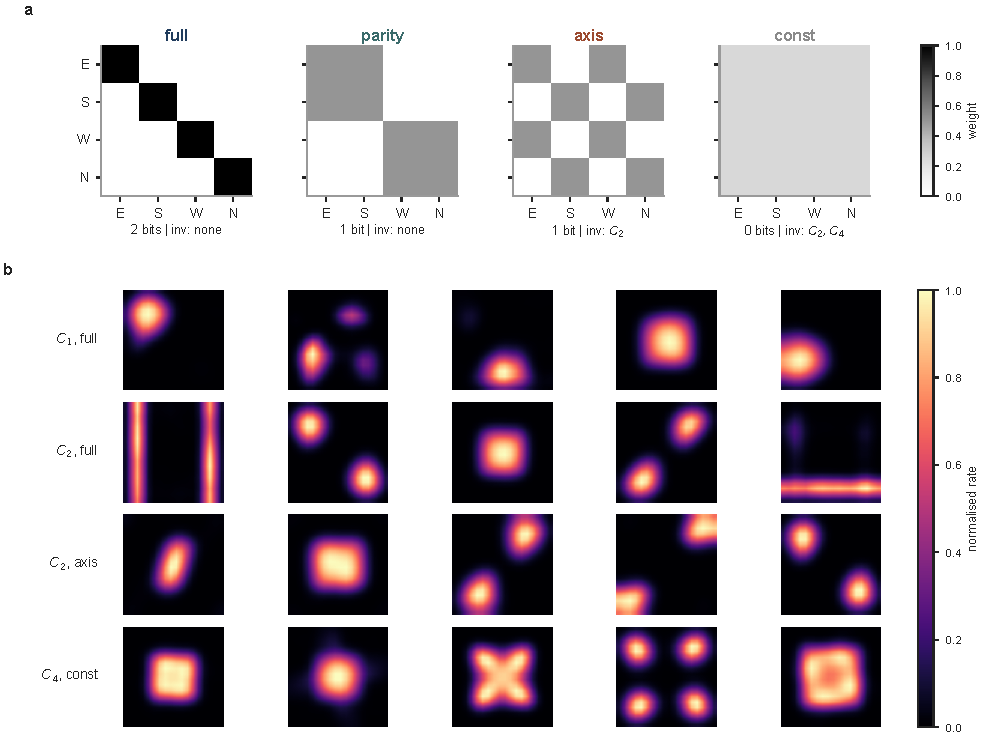
\includegraphics[width=\textwidth]{figures/fig1_setup.pdf}
\caption{\textbf{Design and phenotype.} (\textbf{a}) The four head-direction encodings, as
$4\times4$ transforms of the one-hot heading block $\{$E,S,W,N$\}$; grey level is the matrix
weight. \textit{full} is the identity (two bits); \textit{parity} and \textit{axis} collapse the
compass to one bit with different partitions; \textit{const} discards it. \textit{axis} and
\textit{const} are invariant under the $180^\circ$ rotation and fold the $C_2$ arena;
\textit{const} is the only encoding invariant under the full $C_4$ group. \textit{axis} and
\textit{parity} carry identical information and differ only in invariance. (\textbf{b}) Mean
firing-rate maps (smoothed, peak-normalised) of example units. Fields are single and sharp when
the code does not fold, and repeat at the symmetry-related locations --- once under $C_2$
(\textit{axis} encoding) and four times under $C_4$ (\textit{const}). Units are representative;
the complete unselected set for each condition is given in the Supplementary Information.}
\label{fig:setup}
\end{figure}

The two hypotheses make opposite predictions. If folding tracks how much information the
compass carries, \textit{axis} and \textit{parity} behave alike (Fig.~\ref{fig:setup}a). If
it tracks invariance, \textit{axis} folds and \textit{parity} does not.

\subsection{Predictive learning grows place cells, and symmetry makes them repeat}

Trained on prediction alone, the networks develop units with localised spatial firing fields,
the place cells reported for this objective by \citet{levenstein2024}
(Fig.~\ref{fig:setup}b). In the asymmetric arena under the full compass, about $480$ of the
$500$ units carry a place field (a median of about two fields per unit). The effect of symmetry is visible in the rate maps
before any decoder is applied. When the arena is symmetric and the head-direction encoding is
invariant to that symmetry, the fields repeat: a unit in the $C_2$ arena under \textit{axis}
fires at a location and again at its $180^\circ$ image, and a unit in the $C_4$ arena under
\textit{const} fires at all four $90^\circ$ copies. A single unit reports every member of a
symmetry orbit as the same place. The sections that follow quantify this and isolate what
controls it.


\subsection{Invariance, not information, folds the code}

Under folding onto $X/G$ the population state satisfies $h(x) = h(R^2x)$, so no decoder can
recover which element of the orbit $\{x, R^2x\}$ produced it. We therefore train a linear
decoder for \emph{orbit phase}, holding out whole orbits across cross-validation folds so the
decoder must generalise a phase direction to positions it has never seen. Chance is $0.500$.

\begin{table}[t]
\centering
\caption{Orbit-phase decoding accuracy (chance $=0.500$). $n=10$ per cell for s1 and s2,
$n=8$ for s4.}
\label{tab:phase}
\begin{tabular}{lcccc}
\toprule
arena & \textit{full} & \textit{parity} & \textit{axis} & \textit{const} \\
\midrule
s1 ($C_1$, no symmetry) & 0.981 & 0.972 & 0.971 & 0.966 \\
s2 ($C_2$)              & 0.978 & 0.955 & \textbf{0.552} & \textbf{0.552} \\
s4 ($C_4$)              & 0.984 & 0.933 & \textbf{0.544} & \textbf{0.521} \\
\bottomrule
\end{tabular}
\end{table}

In the $C_2$ arena, \textit{axis} and \textit{parity} --- carrying identical information ---
differ by $0.403$ in phase accuracy. The separation is complete: every \textit{parity} network
scores above every \textit{axis} network (Mann--Whitney $U=0$, $p = 1.1\times10^{-5}$, the exact
two-sided floor at $n=10$ vs.\ $10$; $p = 3.2\times10^{-5}$ after Bonferroni correction across
the three arenas). In the $C_1$ arena, where there is no symmetry to collapse onto, the same two
encodings are indistinguishable ($\Delta = 0.000$, $p = 0.97$). The $C_1$ null is what licenses
the causal reading: \textit{axis} does not degrade spatial coding in general, it degrades it
exactly when the arena has a symmetry under which \textit{axis} is invariant.

The chance-level reading of the folded codes is not an artefact of using a linear decoder. On
the same population states, a $k$-nearest-neighbour decoder and a multi-layer perceptron also
sit at chance for the invariant encodings in the $C_2$ arena (\textit{axis}: $0.537$ and
$0.535$; \textit{const}: $0.531$ and $0.531$; $n=6$), and both recover orbit phase for the
non-invariant encodings (\textit{full} and \textit{parity}, every network $\ge 0.90$). The
orbit-phase information is absent from the folded code, not merely inaccessible to a linear
readout.

None of the folded networks has simply stopped representing space. For 104 of the 112 networks,
$\max(R^2_{\text{raw}}, R^2_{\text{domain}}) \ge 0.81$: the folded codes still linearly encode
position \emph{within the fundamental domain}, they have merely discarded which copy of it the
animal occupies (Fig.~\ref{fig:manifold}). The eight exceptions are \textit{const} in the $C_4$
arena, which fails both $C_2$-based readouts ($R^2_{\text{raw}} = -0.069$,
$R^2_{\text{domain}} = -0.589$) not because it has stopped coding space but because it is folded
by the \emph{full} $C_4$ group, which a $C_2$ decoder cannot see; the next section resolves it.

\begin{figure}[t]
\centering
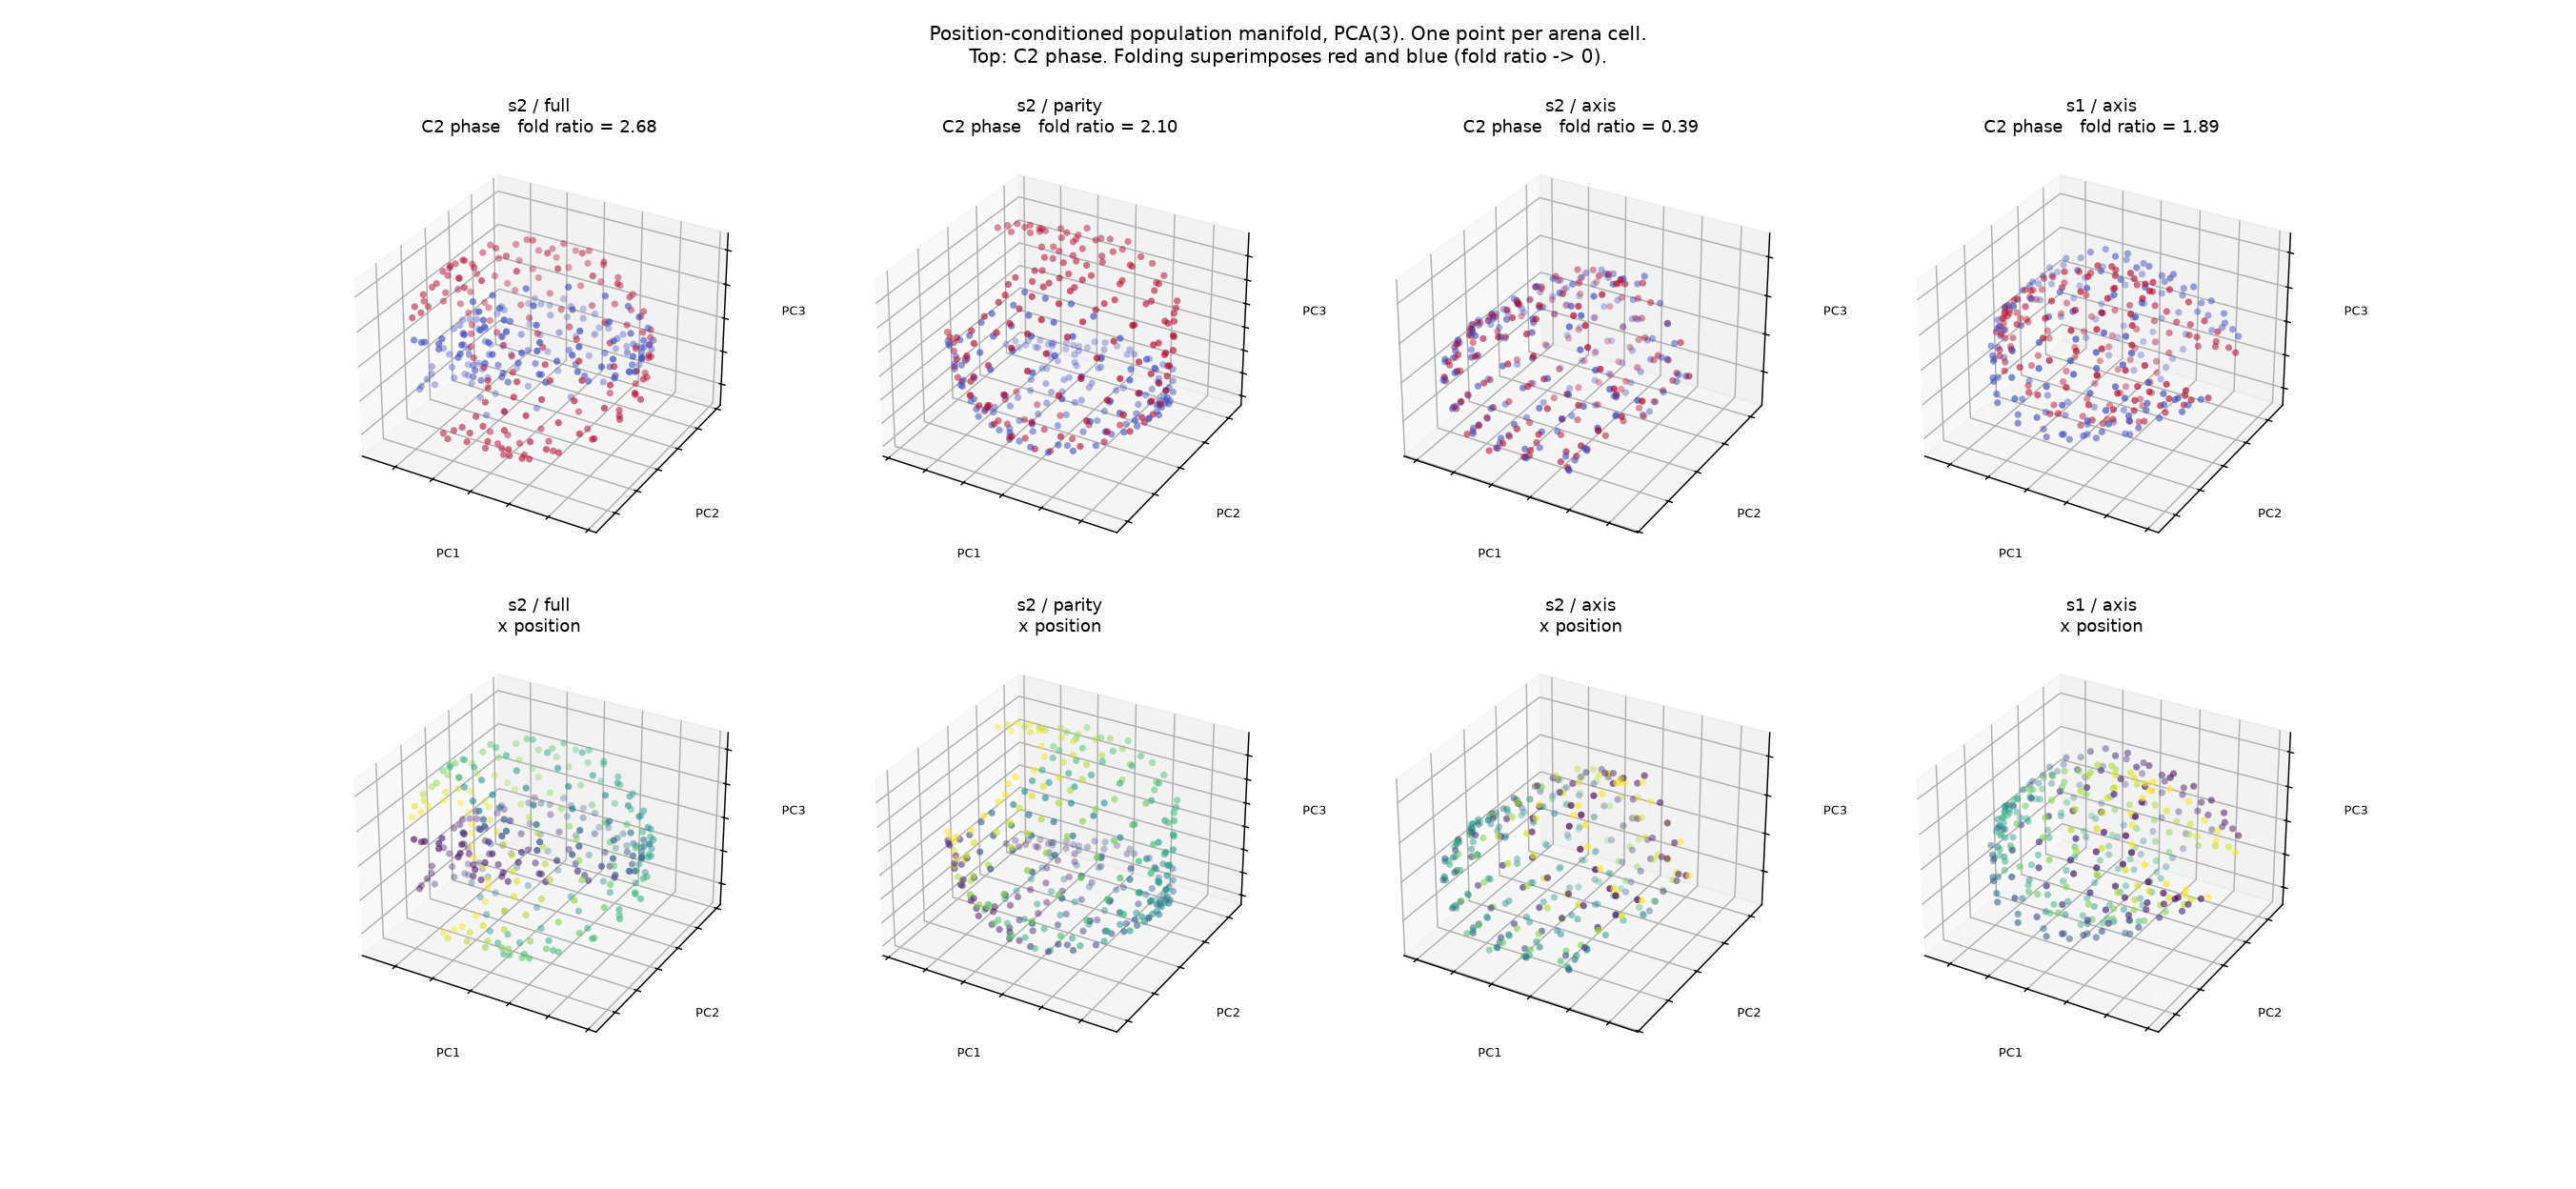
\includegraphics[width=\textwidth]{figures/manifold_s2.png}
\caption{\textbf{The fold, seen geometrically.} Position-conditioned population manifold of a
representative network (one point per arena cell, PCA to three dimensions), coloured by $C_2$
orbit phase. Under \textit{full} and \textit{parity} the two phases occupy separate regions;
under \textit{axis} in the $C_2$ arena they superimpose. The fold ratio --- distance between a
cell and its $180^\circ$ image, in units of the distance to a spatial neighbour --- is 2.68,
2.10 and 0.39 for the three $C_2$-arena encodings shown, and 1.89 for \textit{axis} in the
$C_1$ arena, where the same encoding folds nothing. The ratio is a property of the full hidden
space, not of the linear projection: the folded \textit{axis}/$C_2$ case reads below one and
every non-folded case above one under distance-preserving nonlinear embeddings (Isomap, t-SNE)
as well as PCA. We reduce with PCA because the claim is metric --- two positions coincide ---
and unlike neighbour-graph embeddings PCA preserves distances rather than reshaping them.}
\label{fig:manifold}
\end{figure}

\subsection{The $C_4$ arena reproduces the group-theoretic ceiling}

A code folded onto $X/G$ cannot name the element of an orbit, only the coset, so a $|G|$-way
phase decoder is bounded above by $1/|G|$. Reading the $C_4$ arena through its own quotient
(four-way phase, chance $0.250$) recovers this pattern (Table~\ref{tab:c4}). \textit{const} is
the only $C_4$-invariant encoding, and the only one to fall to the $C_4$ floor ($0.275$, just
above $0.250$). \textit{axis} is $C_2$- but not $C_4$-invariant, and sits near the $C_2$ ceiling
of $0.5$ ($0.482$). The folded values sit within a few percent of their predicted floors rather
than exactly on them; the small residual is consistent with finite-sample decoding, and the
decisive quantity is which floor each encoding falls to, not the residual.

This also resolves \textit{const} in the $C_4$ arena. Read through the $C_4$ quotient it is
plainly a live spatial code --- its $C_4$ fundamental-domain $R^2$ is $+0.646$ (minimum $+0.535$
across all sixteen s4 networks) --- and its four-way phase accuracy of $0.275$ sits at the $C_4$
chance floor. What looked like a dead code under a $C_2$ readout is a code folded onto a larger
quotient than the readout was built to see. We flag this because a $G$-folded code and a code
that has stopped representing space are easy to confuse, and only the second is a failure.

\begin{table}[t]
\centering
\caption{$C_4$ four-way phase decoding in the s4 arena (chance $= 0.250$).}
\label{tab:c4}
\begin{tabular}{lccc}
\toprule
encoding & invariance & measured & predicted ceiling \\
\midrule
\textit{full}   & none          & 0.918 & --- \\
\textit{parity} & none          & 0.860 & --- \\
\textit{axis}   & $C_2$ only    & \textbf{0.482} & 0.500 \\
\textit{const}  & $C_2$ and $C_4$ & \textbf{0.275} & 0.250 \\
\bottomrule
\end{tabular}
\end{table}

\subsection{The ceiling is set by the inputs; the objective decides whether it is reached}

None of this requires a trained network to predict. Call two states $(x,h)$ and $(x',h')$
\emph{input-equivalent} if they produce the same $7\times7$ observation and the same HD encoding.
A code is a function of its inputs, so no decoder can separate input-equivalent states, and phase
decoding is bounded above by

\begin{equation}
\mathrm{acc}_{\max} \;=\; \tfrac12 + \tfrac12 \, \Pr_{(x,h)}\!\big[\,(x,h) \not\sim (R^2x,\, h+2)\,\big],
\label{eq:bound}
\end{equation}

the fraction of orbit pairs the input distinguishes. Evaluating the right-hand side on the arenas
themselves --- enumerating all $324\times4$ states and hashing their observations --- takes no
training at all.

\begin{table}[t]
\centering
\caption{The bound of Eq.~\ref{eq:bound}, computed from the arenas with no free parameters,
against the trained networks. Every encoding falls to the accuracy its input-distinguishability
predicts; the mean absolute error across the twelve cells is $0.031$. (We report the bound as a
bound, not a fit: the predicted values are near-degenerate --- clustered at $1.0$ and at the
folding floors --- so a correlation coefficient across cells would merely register that
separation.)}
\label{tab:bound}
\begin{tabular}{llccc}
\toprule
arena & encoding & distinguishable & predicted & measured \\
\midrule
s1 & \textit{full} / \textit{parity} & 1.000 & 1.000 & 0.981 / 0.972 \\
s1 & \textit{axis} / \textit{const}  & 0.934 & 0.967 & 0.971 / 0.966 \\
s2 & \textit{full} / \textit{parity} & 1.000 & 1.000 & 0.978 / 0.955 \\
s2 & \textit{axis} / \textit{const}  & 0.000 & 0.500 & 0.552 / 0.552 \\
s4 & \textit{full} / \textit{parity} & 1.000 & 1.000 & 0.984 / 0.933 \\
s4 & \textit{axis} / \textit{const}  & 0.000 & 0.500 & 0.544 / 0.521 \\
\bottomrule
\end{tabular}
\end{table}

Table~\ref{tab:bound} also settles a number that would otherwise look like a failure. In the
$C_1$ arena \textit{axis} reaches $0.971$ rather than $1.000$ --- because $6.6\%$ of states there
are \emph{accidentally} observationally identical to their $C_2$ partner, putting the bound at
$0.967$. \textit{axis} and \textit{const} sit exactly on it. They were not failing to fold; they
were folding on precisely the ambiguous fraction.

\paragraph{The objective selects the bound.} The inequality is an upper bound, not a prediction:
a network is free to discard information its loss does not reward. This is what the horizon sweep
shows. At $k=0$ the input still separates $1228$ of the $1296$ states under \textit{full} --- the
compass is right there --- yet all four encodings collapse to within $0.005$ of one another
(Table~\ref{tab:horizon}), landing on the \emph{observation-only} bound of $0.500$. The spread
across encodings is $0.0052$ at $k=0$ against $0.427$ at $k=5$ (Fig.~\ref{fig:function}a).

So the compass is not absent under reconstruction; it is \emph{discarded}. Reconstructing
$o_t$ never requires knowing which of two identical-looking places you occupy. Predicting $o_{t+1}$
does, and one step is enough.

\subsection{The fold is resolved by prediction, not by observation}

We repeated the s2 sweep varying only the rollout horizon $k$. At $k=0$ the network's target is
its own current observation at the anchor (verified exactly), i.e.\ a pure autoencoder with the
same architecture and the same head-direction input, but no future to predict.

\begin{table}[t]
\centering
\caption{Orbit-phase decoding in the $C_2$ arena as a function of prediction horizon $k$
(chance $= 0.500$, $n = 6$ per cell).}
\label{tab:horizon}
\begin{tabular}{lccccc}
\toprule
$k$ & \textit{full} & \textit{parity} & \textit{axis} & \textit{const} & \textit{axis} vs \textit{parity} \\
\midrule
0 (autoencoder) & 0.536 & 0.541 & 0.539 & 0.539 & $p = 0.59$ \\
1 & 0.975 & 0.941 & 0.545 & 0.546 & $p = 0.00216$ \\
3 & 0.968 & 0.947 & 0.548 & 0.545 & $p = 0.00216$ \\
5 & 0.978 & 0.953 & 0.553 & 0.551 & $p = 0.00216$ \\
\bottomrule
\end{tabular}
\end{table}

Under reconstruction the full two-bit compass buys nothing: every encoding folds, and all four
sit near chance (Table~\ref{tab:horizon}). These are folded codes, not broken ones --- the
minimum of $\max(R^2_{\text{raw}}, R^2_{\text{domain}})$ across all 24 autoencoder networks is
$0.858$. A single step of prediction restores the effect in full, and extending the horizon to
five adds nothing: the dependence on $k$ is a step, not a gradient.

The reason is that the autoencoder's target is the current observation, which the compass
cannot help predict, so the objective gives the network no reason to integrate self-motion and
the $C_2$-symmetric observation stream determines the code. Prediction of a future observation
requires integrating self-motion across at least one step, and it is that integration which
resolves the symmetry. The control therefore isolates a property of the objective rather than of
reconstruction as such: an objective that does not require self-motion integration does not
recruit the compass, whatever else it reconstructs.

\begin{figure}[t]
\centering
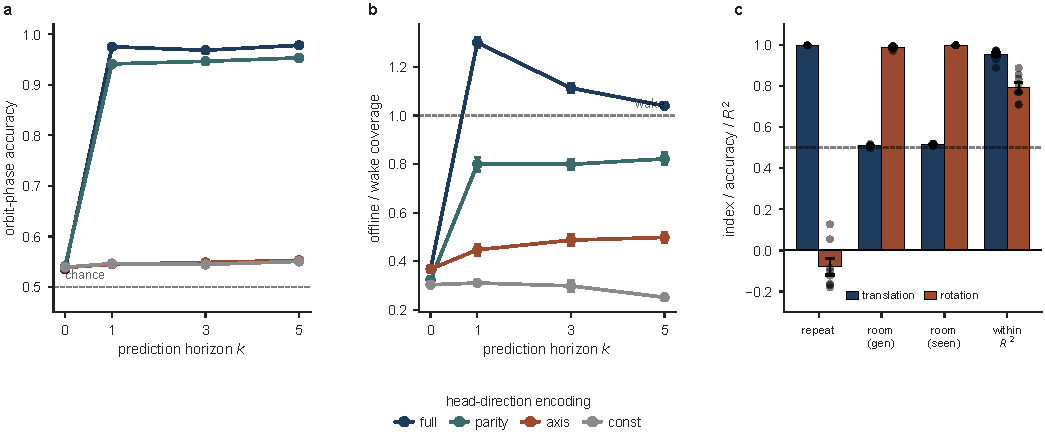
\includegraphics[width=\textwidth]{figures/fig3_function.pdf}
\caption{\textbf{Functional consequences of the fold.} (\textbf{a}) Orbit-phase decoding
accuracy vs prediction horizon $k$ in the $C_2$ arena (chance $0.5$); the non-invariant
encodings (\textit{full}, \textit{parity}) resolve the fold at $k \geq 1$, the invariant ones
(\textit{axis}, \textit{const}) stay near chance. (\textbf{b}) Coverage of the self-generated
offline trajectory as a fraction of a wake path of equal length (dashed line, wake). Both step
up at $k = 1$ and are ordered by how much of the compass the encoding keeps; points are mean
$\pm$ s.e.m., $n = 6$. (\textbf{c}) Place-field repetition across two observationally identical
compartments ($n = 8$ each): under translation the fields repeat and the room is undecodable
(chance $0.5$), under rotation the fields do not repeat and the room decodes; within-room
position ($R^2$) stays high in both. Dots are individual networks.}
\label{fig:function}
\end{figure}

\subsection{Offline replay emerges at the same horizon as symmetry resolution}

A predictive network can be run offline, driven by its own predicted observation in place of a
real one, so that it generates trajectories without moving through the arena
\citep{levenstein2024}. We generated $200$-step offline trajectories from each $C_2$ network and
decoded position with a ridge decoder fit on waking activity (Fig.~\ref{fig:function}b).
For each trajectory we measured the fraction of the arena it covered, relative to a waking
trajectory of the same length; a $200$-step walk visits only $27\%$ of the arena, so the raw
fraction is hard to read on its own.

Offline coverage rose sharply between $k=0$ and $k=1$ and changed little afterwards, tracking
the step in orbit-phase accuracy over the same range. At $k=0$, where the network reconstructs
its current observation, coverage stayed below $37\%$ of waking under every encoding. From
$k=1$ the \textit{full} compass drove trajectories that covered more of the arena than waking
behaviour itself, at $1.30$, $1.11$ and $1.04$ times waking for $k=1$, $3$ and $5$. Coverage
fell as the compass was weakened, from $1.30$ times waking under \textit{full} to $0.80$,
$0.45$ and $0.31$ under \textit{parity}, \textit{axis} and \textit{const}, the same order in
which the code folds. Step-to-step continuity did not follow this ordering and was highest for
\textit{const}, since a network whose state barely moves produces short smooth steps whatever
it represents. Offline generation and symmetry resolution therefore depend on prediction and on
head direction in the same way, and appear at the same horizon.

These offline trajectories are temporally ordered rather than random walks, and only when the
compass is intact. We score sequenceness as the rank correlation between a rollout's
principal-axis position and time, against a circular time-shift null and a cell-identity
shuffle. In the $C_2$ arena the \textit{full} network's offline paths reach a sequenceness of
$0.53$, close to the waking reference of $0.56$ and well above the cell-shuffle floor of $0.25$,
whereas the folded \textit{axis} and \textit{const} encodings fall to that floor ($0.20$ against
$0.17$). Coherent replay, like coverage, requires the head-direction signal the fold discards.

\subsection{The dissociation survives a noisy compass}

The head-direction signal used so far is a noiseless oracle, whereas the biological compass
drifts and is re-anchored by vision. To test whether the fold depends on a perfect signal, we
retrained the $C_2$ networks with the reported heading corrupted: on $30\%$ of steps the compass
was rotated by a random $\pm 90^\circ$ before encoding. The dissociation is preserved. Orbit-phase
decoding is $0.556$ under \textit{axis} and $0.922$ under \textit{parity}, a separation of
$0.367$ that remains complete: every \textit{parity} network scores above every \textit{axis}
network (Mann--Whitney $U = 0$, $p = 0.0022$ at $n = 6$ vs.\ $6$). Relative to the clean
networks the separation narrows only slightly (from $0.403$), driven by a small drop in
\textit{parity} resolution ($0.955 \to 0.922$) while the folded \textit{axis} code is unchanged
($0.552 \to 0.556$). A compass corrupted on a third of steps still folds the same symmetries
it does when clean. (These networks were trained for $30{,}000$ steps rather than
$80{,}000$; the effect is already complete by then.)

\subsection{Two natural readouts fail, in two different ways}

Decomposing each unit's rate map into the four characters of $C_4$ gives an isotypic power
spectrum $P_0 \dots P_3$. Rotational autocorrelation, the quantity used in earlier analyses of
this system, is exactly $\mathrm{RA} = P_0 - P_2$. It is therefore \emph{blind to $C_2$
structure}: invariance under $R^2$ annihilates the odd characters $P_1$ and $P_3$ while leaving
$P_0$ and $P_2$ untouched, so a perfectly $C_2$-folded code and pure noise both read
$\mathrm{RA}\approx0$. Empirically, on a clean 17-network sweep, RA cannot separate s2 from s1
($p = 0.056$), whereas odd power $P_1 + P_3$ separates them completely ($p = 0.0079$, the exact
floor at $n=5$ vs.\ $5$).

Odd power, however, is itself confounded. Under \textit{axis} it falls in the $C_1$ arena too,
where there is no symmetry: the drop $\mathrm{odd}(\textit{parity}) - \mathrm{odd}(\textit{axis})$
is $0.095$ in s1, $0.111$ in s2 and $0.112$ in s4, so $85\%$ of the s4-sized effect is present
where nothing can fold, and it separates completely in s1 ($p = 1.8\times10^{-4}$) --- a
confident report of a fold that does not exist. Odd power conflates genuine collapse onto the quotient with the encoding merely
reshaping the rate-map spectrum. Orbit-phase decoding is immune to that and returns a clean null.

We therefore report phase decoding as the primary readout and the isotypic spectrum as a
secondary, descriptive one. We note this explicitly because the confounded readout would have
supported the same qualitative conclusion, by an argument that does not hold.

\subsection{Folding leaves a reproducible spatial map intact}

Because the folded encodings decode orbit phase near chance (about $0.55$, reliably just above
the $0.5$ floor but far below the $\sim\!0.95$ of the non-invariant encodings), we asked whether they had learned a
spatial map at all, or whether ablating the compass had degraded the representation more
broadly. Two measures argue that the map is intact (Fig.~\ref{fig:fold}c,d). Spatial
representational similarity, the Spearman correlation between neural distance and Euclidean
distance across pairs of positions, fell as the compass was ablated, from $0.70$ under
\textit{full} to $0.32$ under \textit{const} in the $C_1$ arena, and lower still in the
symmetric arenas. This is the expected consequence of folding: a position and its group image
sit on top of one another in the neural space while lying far apart in the arena, weakening the
correlation between the two distances. The correlation between the position-conditioned codes of
independently trained networks behaved oppositely and stayed above $0.96$ under every encoding
in every arena, and $448$ of the $500$ units retain a place field under \textit{const} in the
$C_1$ arena, falling to about $318$ in the $C_4$ arena. A folded code is therefore reproducible rather than degenerate, and the compass
governs how the map is laid out rather than whether one forms.

The collapse can also be read in the metric used to score remapping in the hippocampus. The
population-vector correlation between a position and its symmetry image \citep{leutgeb2005} ---
near one when the two share a representation, near zero when the code separates them --- is
$0.98$ under the invariant encodings in the $C_2$ and $C_4$ arenas and about $0.28$ under
\textit{full}, with the matched non-invariant encoding intermediate (\textit{parity}, $0.58$ in
$C_2$; $n = 10$ per encoding). By this measure the network fails to remap between
symmetry-related locations exactly when the compass is invariant under the symmetry --- the two
copies are written as one place --- whereas with a full compass they are separated as strongly as
unrelated positions. The same invariant encoding gives a weaker correlation in the $C_1$ arena
($0.71$ for \textit{axis}), where there is no arena symmetry to complete the fold.

\begin{figure}[t]
\centering
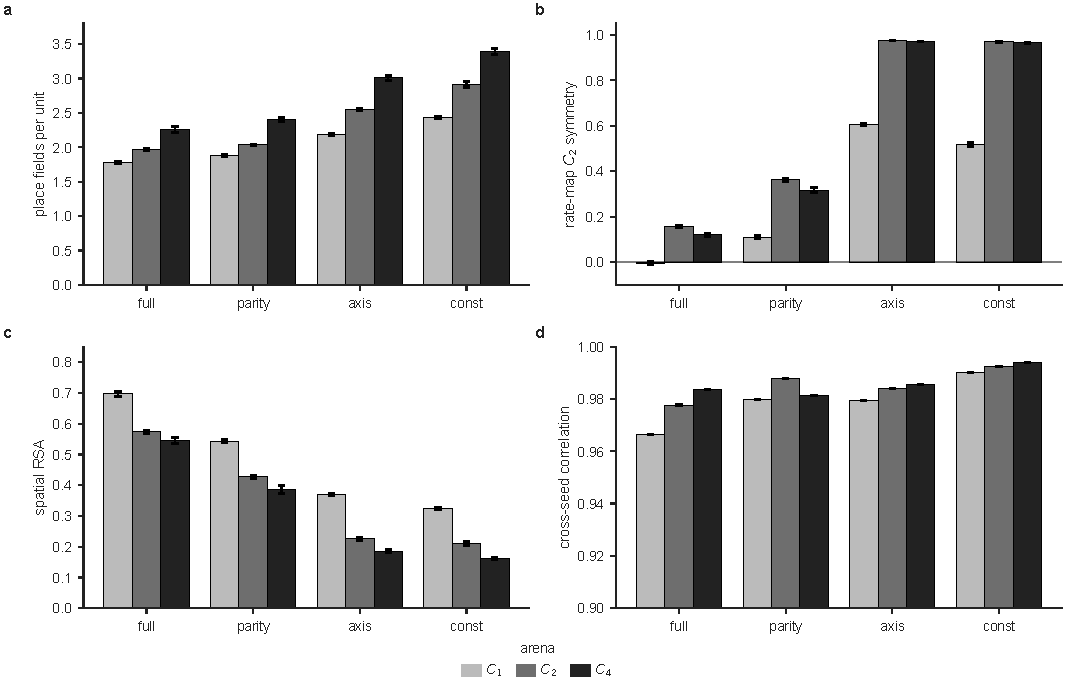
\includegraphics[width=\textwidth]{figures/fig2_fold.pdf}
\caption{\textbf{Quantifying the fold.} (\textbf{a}) Mean place fields per unit; rises with both
arena symmetry and encoding invariance, but also in the $C_1$ arena where nothing folds, so
field count alone is confounded. (\textbf{b}) Rate-map $C_2$ symmetry index (correlation of a
unit's map with its $180^\circ$ rotation), the fold-specific readout; it saturates near $0.97$
only when the encoding is invariant to the arena's symmetry. (\textbf{c}) Spatial
representational similarity falls as the encoding is ablated and as arena symmetry increases,
the signature of collapse onto the quotient. (\textbf{d}) Cross-seed correlation between
independently trained networks stays above $0.96$ throughout ($y$ zoomed to $0.9$--$1.0$): the
fold is reproducible, not degenerate. Arenas $C_1/C_2/C_4$; bars are mean $\pm$ s.e.m.\ over
networks ($n = 10$ per encoding for $C_1$ and $C_2$, $n = 8$ for $C_4$).}
\label{fig:fold}
\end{figure}

\subsection{Folding multiplies place fields and imprints the arena's symmetry on each map}

The fold is visible cell by cell, not only in the population decoder. We characterised every
unit's firing-rate map and counted its place fields (Fig.~\ref{fig:fold}a). Fields per unit
rise with both arena symmetry and encoding invariance, from $1.78$ under \textit{full} in the
$C_1$ arena to $3.39$ under \textit{const} in the $C_4$ arena. On its own this count is a
confounded readout: it rises even in the $C_1$ arena, where nothing can fold ($2.44$ fields
under \textit{const} against $1.78$ under \textit{full}), because a more invariant encoding
yields more multi-peaked units regardless of symmetry. The fold-specific question is whether
the extra fields sit at group-related positions. We measure this as the correlation between a
unit's rate map and its own $180^\circ$ rotation, a per-cell index of $C_2$ symmetry
(Fig.~\ref{fig:fold}b). The index saturates near $0.97$ exactly when the encoding is
$C_2$-invariant and the arena is symmetric (\textit{axis} and \textit{const} in the $C_2$ and
$C_4$ arenas), while the matched non-invariant encoding stays low (\textit{parity}, $0.36$ in
$C_2$) and \textit{full} stays low throughout ($\le 0.16$). An invariant encoding alone induces
partial symmetry even in the $C_1$ arena ($0.61$ for \textit{axis}), which the arena's own
symmetry then completes. The four-fold version of the index reaches $0.97$ only for
\textit{const} in the $C_4$ arena, the single fully $C_4$-invariant condition. Each map
acquires precisely the symmetry the compass cannot break.

Scored by the criteria applied to real recordings, the trained population is a realistic
mixture rather than a bank of identical units: $76$--$96\%$ of units qualify as place cells
(Skaggs spatial information above threshold) and about $30\%$ are border-modulated (a third or
more of their rate-map mass in the outer ring), a composition that is stable across encodings and
arenas (Supplementary Information). Folding therefore multiplies fields and rearranges where they sit without changing the
cell-type makeup of the map --- the multi-field, spatially repeating cells it produces are the
in-silico counterpart of the repeated place fields recorded in symmetric environments
\citep{muller1987, grieves2016}.

\subsection{The same dissociation appears across observationally identical compartments}

Head direction should resolve rotational but not translational symmetry, and this can be tested
in the geometry used to study repeated place fields in rodents. We built two closed $6\times6$
compartments joined by a corridor and gave them identical interior landmarks, so that the two
rooms produced the same set of egocentric views; across all $144$ combinations of location and
heading the observations coincided exactly. In one arrangement the rooms were related by a
translation, under which the compass reads the same in both; in the other by a rotation, under
which it does not. We trained networks on each arrangement and, for every network, decoded which
room the animal occupied and measured whether individual units repeated their firing fields
between the rooms (Fig.~\ref{fig:function}c).

The two arrangements gave opposite results ($n=8$ networks each). Under translation the fields
repeated almost exactly across the rooms (repetition $0.997$) and the room could not be decoded
even by a nearest-neighbour classifier tested on cells it had already seen ($0.515$, chance
$0.5$), so the network folded the two identical rooms onto one map. Under rotation the
repetition vanished (repetition $-0.080$) and the room decoded perfectly ($0.998$). Position
within a room decoded well in both arrangements ($R^2 = 0.95$ and $0.79$), so neither network
had stopped representing space. Every translation network separated from every rotation network
on all four measures (Mann--Whitney $p = 1.6\times10^{-4}$, the exact two-sided floor at $n=8$
vs.\ $8$). \citet{grieves2016} reported this same contrast in CA1, and here it follows from
nothing but the group action of the arena on the compass.


\section{Discussion}

The result is a statement about group actions rather than about information channels. A
self-motion signal resolves exactly those symmetries under which it is not itself invariant.
Head direction is blind to translation --- translating the world does not change a compass
reading --- and therefore cannot disambiguate translationally repeated compartments, whereas it
is not blind to rotation and can disambiguate rotationally related ones.

\subsection*{The dissociation exists in the animal data}

\citet{spiers2015} recorded CA1 place cells in four visually identical compartments arranged in a
row off a connecting corridor, and found ``a high degree of spatial repetition with a slight
degree of rate-based discrimination''. Those compartments are translationally related, and the
authors conclude that ``path integration is not used, or at least not spontaneously'' to separate
them. \citet{grieves2016} then ran the same four compartments in two arrangements. Parallel, all
facing the same way and therefore translationally related: ``place cells often exhibited repeated
fields''. Radial, at $60^\circ$ to one another and therefore rotationally related:
``significantly less place field repetition was apparent'' (all $p < 0.0001$). The dissociation
survived removal of the orientation landmark, so it is not carried by extra-maze vision, and the
authors attribute it to ``directional information derived from the animal's self-motion'',
hypothesising the head-direction system as the source.

Our result supplies the reason. A compass is \emph{invariant} under translation and
\emph{equivariant} under rotation. The input process is therefore $G$-equivariant in the parallel
arrangement and not in the radial one, so a predictive code must fold onto the quotient in the
first case and may lift it in the second. Repetition is not a failure of the hippocampus; it is
what a predictive code must do when its self-motion signal cannot see the symmetry.

Two things follow that the animal data cannot establish. First, the effect is a property of
\emph{invariance}, not of how much the compass tells you: two encodings carrying the same single
bit dissociate completely (Table~\ref{tab:phase}). Second, it is a property of \emph{prediction}:
under a matched reconstruction objective the compass is inert (Table~\ref{tab:horizon}), so head
direction cannot disambiguate compartments unless the objective forces the network to integrate
it. Whether a purely reconstructive circuit would show repetition even in the radial arrangement
is, to our knowledge, untested in animals.

The account also yields a lesion prediction, with a dose attached. Lesions of the anterodorsal
thalamus degrade the head-direction signal and destabilise hippocampal place fields
\citep{calton2003}. We predict that degrading the compass should bring field \emph{repetition}
into the \emph{radial} arrangement, where intact animals show little, because without direction
rotation joins translation as a symmetry the animal cannot resolve. The robustness control sets
the threshold high, though: in the model a compass corrupted on $30\%$ of steps still resolves
the fold, and full repetition appears only in the \textit{const} limit of near-total directional
loss (which folds the $C_2$ arena to near chance, Table~\ref{tab:phase}). A partial ADN lesion
should therefore produce partial repetition, graded by how much of the head-direction signal
survives.


\subsection*{What the model reproduces, and what it does not}

\begin{table}[t]
\centering
\small
\setlength{\tabcolsep}{4pt}
\caption{The model against the animal literature. ``Reproduced'' means the model shows the
phenomenon without being fitted to it; ``absent'' means the phenomenon cannot exist in this
architecture and we do not claim it.}
\label{tab:bio}
\begin{tabular}{p{0.29\textwidth}p{0.22\textwidth}p{0.28\textwidth}p{0.11\textwidth}}
\toprule
observation in animals & source & in this model & verdict \\
\midrule
Fields repeat across translationally related identical compartments; path integration does not
separate them
& \citet{spiers2015} & translation leaves the compass invariant, so the code folds onto $X/G$
& reproduced \\[4pt]
Repetition in parallel compartments, markedly less in radial ones; survives removal of the
orientation landmark; attributed to self-motion
& \citet{grieves2016} & rotation makes the compass equivariant, so the code lifts
& reproduced \\[4pt]
Multi-field firing increases with the rotational symmetry of the arena
& \citet{muller1987, knierim1995} & folding onto $X/G$ makes one unit fire at all $|G|$ orbit-mates
& reproduced \\[4pt]
Head-direction input is required for a stable map; ADN lesions destabilise place fields
& \citet{calton2003} & the \textit{const} encoding folds the $C_2$ arena to near chance
& consistent \\[4pt]
Head direction plus recurrence plus prediction are needed for offline replay
& \citet{levenstein2024} & offline trajectories exceed the coverage of a wake path of equal
length only with the full compass and $k \ge 1$; coverage falls monotonically as the compass
is ablated ($1.30 \to 0.80 \to 0.45 \to 0.31 \times$ wake), and the autoencoder never leaves
$0.37\times$. Replay appears at the same horizon as symmetry resolution and improves no
further with a longer one
& reproduced \\[4pt]
Rate remapping: a slight rate-based discrimination between otherwise repeated fields
& \citet{spiers2015} & absent. In the parallel arrangement the fields repeat perfectly
(repetition $+0.997$) and the compartment is not decodable even by a nearest-neighbour
readout at cells it has already seen ($0.515$, chance $0.5$). The fold is complete; the
animals retain a residual rate signal that this network does not
& not reproduced \\[4pt]
Grid cells on a toroidal population manifold, invariant across environments and sleep
& \citet{gardner2022toroidal} & no grid cells (gridness $\le 0.08$); the torus cannot exist here
& absent \\[4pt]
Head-direction cells lie on a ring manifold that matures before place and grid coding
& \citet{taube1990, langston2010} & head direction is supplied as a four-point input, not learned
& absent \\
\bottomrule
\end{tabular}
\end{table}

The two rows marked \emph{absent} are architectural, not empirical: head direction enters this
network as an oracle input rather than being learned, and no non-negativity constraint is imposed,
which is the condition under which hexagonal grids emerge in trained path integrators
\citep{sorscher2023unified}. Nothing here bears on the ring or toroidal manifolds of entorhinal
cortex, and we make no claim about them.

The objective control constrains the mechanism further: a matched autoencoder with the same
wiring and the same compass folds every encoding alike ($p = 0.59$), which rules out the fold
being a property of the input pipeline rather than of the learning. It is an objective that
requires predicting a future observation, not reconstructing the present one, that recruits the
compass.

\subsection*{Relation to other models of the spatial code}

The parallel-versus-radial dissociation is a discriminating test among models of place-cell
firing, because the two arrangements are built from the same compartments and are locally
identical in both. A model that fixes firing from local sensory or boundary geometry alone must
therefore predict the same repetition in each: the boundary-vector account \citep{hartley2000},
in which a field is a fixed function of the distances to walls, gives identical fields wherever
the local geometry recurs, parallel or radial. A reconstruction objective behaves the same way
for the same reason, and our autoencoder control confirms it --- with the compass held identical
it folds every encoding alike. Continuous-attractor path integrators \citep{burak2009,
sorscher2023unified} build the metric in by construction and do not speak to what happens when
observations alias. The successor representation \citep{stachenfeld2017, momennejad2017successor}
is predictive, but over a state space that is supplied rather than inferred from aliased
observations, so whether two symmetric compartments are one state or two is an assumption, not a
result (Table~\ref{tab:models}).

What predictive learning adds is a derivation. Trained only to predict its next view from
self-motion, the network folds or lifts the identical compartments according to whether the
compass is invariant under the arrangement's symmetry, reproducing the animal dissociation from a
single group-theoretic principle rather than fitting it. The contribution is therefore not that
prediction grows place cells \citep{levenstein2024}, but that it specifies \emph{when} the
spatial code collapses under symmetry and when it does not --- a question the other model classes
leave open.

\begin{table}[t]
\centering
\small
\setlength{\tabcolsep}{4pt}
\caption{Where models of the spatial code stand on the symmetry dissociation. The decisive column
is the last: the parallel and radial arrangements are locally identical, so any model that reads
firing from local geometry or the current observation predicts the same repetition in both, and
cannot produce the dissociation \citet{grieves2016} observed.}
\label{tab:models}
\begin{tabular}{p{0.30\textwidth}p{0.15\textwidth}p{0.18\textwidth}p{0.25\textwidth}}
\toprule
model class & fields learned from experience & repetition in identical rooms &
parallel-vs-radial dissociation \\
\midrule
Continuous attractor / path integration \citep{burak2009, sorscher2023unified}
& metric built in & not addressed & no \\[3pt]
Boundary-vector / geometry \citep{hartley2000}
& partly & yes & no --- predicts repetition in both \\[3pt]
Successor representation \citep{stachenfeld2017}
& yes (predictive) & depends on the given state space & not addressed \\[3pt]
Reconstruction / autoencoder (this work, control)
& yes & yes & no --- folds both ($p=0.59$) \\[3pt]
Predictive RNN \citep{levenstein2024}, this work
& yes (emergent) & yes & \textbf{yes}, set by HD invariance \\
\bottomrule
\end{tabular}
\end{table}

\paragraph{Limitations.} The arenas are discrete $18\times18$ grids with four headings, so the
head-direction ``ring'' has four points and no continuous ring topology; nothing here speaks to
the ring or toroidal manifolds reported in entorhinal cortex \citep{gardner2022toroidal}. The networks
develop place-like but not grid-like tuning (gridness over the 100 most spatially tuned units:
mean $-0.35$, maximum $+0.08$, none above the conventional $0.3$ threshold), which is expected
given that head direction is supplied as an input rather than learned and that no
non-negativity constraint is imposed \citep{sorscher2023unified}; the toroidal code of
\citet{gardner2022toroidal} cannot exist in this model, and we do not claim it. The
head-direction signal is a noiseless oracle, whereas the biological compass drifts and is
re-anchored by vision; a control that corrupts the compass on $30\%$ of steps (Results) leaves
the dissociation intact, but a fully learned, continuously drifting compass is not tested here.
We also tested whether
population-manifold topology crystallizes before metric geometry, a proposed developmental
ordering. With a shuffle-null Betti estimator the effect does not hold in these arenas:
position is linearly decodable at $R^2 = 0.79$ in the untrained network, metric geometry
develops gradually. Loop topology is readout-dependent: the linear PCA-6 estimator does not
reliably recover it, yet a spectral (Laplacian) embedding recovers the annulus's single loop in
every network and the open arena's trivial topology, both under-detected by PCA-6
(\texttt{topology\_robustness.csv}). The two-loop theta and figure-8 arenas are not cleanly
recovered by any embedding --- the higher-dimensional linear reduction that occasionally finds
them also hallucinates a loop in the open arena. Simple loop topology is thus present but visible
only through a nonlinear readout, and higher-genus topology is not reliably recovered, so we make
no strong topology-before-geometry claim. The place fields track the animal's current position rather
than a future one: rebuilding each rate map on the position up to five steps ahead does not
sharpen it at any prediction horizon, so the network's predictive character is expressed in its
offline replay rather than in a spatial lead of its fields (though the discrete one-cell-per-step
grid would not resolve a sub-cell anticipatory shift). All results use a single architecture (hidden size $500$,
prediction horizon $k=5$) at one arena size; the horizon sweep shows the fold is present from
$k=1$ and the initialisation study varies the recurrent weights, but hidden size and arena size
are not swept. The architecture has no excitatory--inhibitory separation.
Finally, symmetry here is a property of the landmark layout, not of the arena geometry, which is
square and therefore $C_4$-symmetric in every condition.

\subsection*{Outlook}

The broader appeal of predictive learning is that a single, domain-general objective --- predict
the next observation --- grows structured spatial representations with no hand-built spatial
prior, in artificial networks as in the hippocampus \citep{levenstein2024, stachenfeld2017}. What
this study adds is that the geometry of the learned code is then set by the symmetry structure of
the agent's interaction with the world --- the group action of the environment on the self-motion
signal --- rather than by the architecture. That makes the paradigm a controlled developmental
probe. Because the representation is learned rather than wired in, each factor that shapes it in
an animal, and is there confounded or fixed, becomes a variable that can be turned on its own: the
geometry of the enclosure, including irregular and non-convex ones; the information content and
invariance of the self-motion signal, as here; the locomotor policy and the trajectory statistics
it induces; and the task the agent is trained under. Charting how the code changes along these
axes is a way to ask which features of an environment and an agent are responsible for which
features of the representation.

Architecture is a variable of the same kind. The present network receives head direction as an
oracle input and places no non-negativity constraint on its units, and it accordingly grows
place-like but not grid-like tuning; hexagonal grids emerge in trained path integrators precisely
when those constraints are imposed \citep{sorscher2023unified}. Progressively more biological
designs --- a head-direction signal that is learned and allowed to drift rather than supplied,
non-negative rates, separate path-integration and sensory streams, and modules for planning ---
would let one ask which ingredients are necessary for the joint emergence of place and grid cells
and for the developmental order in which they appear. The aim of such a program is to turn the
catalogue of spatial cell types into a set of consequences that follow from an objective, an
architecture, and an experience, of which the symmetry-driven fold reported here is one.

\section{Methods}

\paragraph{Architecture and training.} We use \texttt{pRNN\_th} \citep{levenstein2024} unchanged:
a layer-normalised recurrent cell, hidden size 500, truncation $T = 200$, rollout horizon $k=5$
unless stated, observation size 147 ($7\times7\times3$), action size 5. Training uses RMSprop
($\alpha = 0.95$, $\epsilon = 10^{-6}$) with four parameter groups at per-group learning rates
$\lambda\sqrt{1/H}$ for $W_{\text{rec}}, W_{\text{out}}$, $\lambda\sqrt{1/(n_{\text{obs}} +
n_{\text{act}})}$ for $W_{\text{in}}$ and $0.1\lambda$ for the bias, with bias-only weight decay;
$\lambda = 2\times10^{-3}$, batch size 8, gradient clipped per model to norm 1, 80{,}000 steps.

\paragraph{Arenas.} $18\times18$ MiniGrid arenas (324 positions) with landmark layouts of $C_1$,
$C_2$ and $C_4$ rotational symmetry. The observational discriminability index (ODI; the Spearman
correlation between heading-averaged observation distance and spatial distance across all pairs
of positions) is \emph{not} matched across the three arenas, and cannot be: symmetric landmarks
make distinct positions observationally identical, so discriminability necessarily falls with
symmetry order. Measured over all 324 positions, $\mathrm{ODI} = 0.336$ ($C_1$), $0.288$ ($C_2$),
$0.262$ ($C_4$). An earlier report of these arenas described them as ``matched at
$\mathrm{ODI}=0.336$''; that value is the $C_1$ arena's ODI alone.

This does not confound the results, for two reasons. The decisive contrast --- \textit{axis} vs.\
\textit{parity} --- is made \emph{within} one arena, on the same trajectories, so the observation
stream and its ODI are identical between the two arms; the only difference is a $4\times4$ matrix
on the heading block. And across arenas, ODI does not predict the readout: with a full compass,
phase decoding is $0.981$, $0.978$ and $0.984$ for $C_1$, $C_2$, $C_4$ (Pearson $r=-0.37$ against
ODI, $p=0.76$, $n=3$ arenas), with the least discriminable arena scoring highest. Trajectories: 10{,}000 per
arena, 200 steps, random start position and heading, random-walk policy.

\paragraph{Head-direction encodings.} The heading block of the action vector is left-multiplied
by a fixed $4\times4$ matrix: identity (\textit{full}); $\tfrac12(I + P^2)$ where $P$ is the
cyclic shift (\textit{axis}); the block-averaging matrix pairing $\{E,S\}$ and $\{W,N\}$
(\textit{parity}); and $\tfrac14\mathbf{1}\mathbf{1}^\top$ (\textit{const}). Column sums are
preserved, so activation magnitude is unchanged. Entropies under a uniform heading prior are
$2, 1, 1, 0$ bits.

\paragraph{Ensemble training.} All networks sharing a computation graph (arena, encoding and seed
all leave it unchanged; the horizon $k$ does not) are trained as a single job using
\texttt{torch.func.stack\_module\_state} with \texttt{vmap(functional\_call)}, which lowers every
per-model matrix multiply to one batched multiply and makes the kernel-launch count independent
of the number of models. Forward passes are bit-exact against separate runs; gradients are
bit-exact with noise disabled and agree to $2.3\times10^{-10}$ absolute with the production noise
on (\texttt{bmm} reassociation). Per-model gradient clipping, the four-group RMSprop and the
sum-of-per-model-means loss are all preserved; each is checked against the reference
implementation by test.

\paragraph{Orbit-phase decoding.} Hidden states are collected over 20{,}000 timesteps and averaged
per position. Orbits are $\{x, R^2x\}$ under the $180^\circ$ rotation (or the four-element $C_4$
orbits where stated); the arena side is even, so no rotation has an integer fixed point and every
orbit has exactly $|G|$ cells. Phase labels are balanced, and cross-validation folds hold out
whole orbits (\texttt{GroupKFold}), so the decoder must generalise a phase direction rather than
memorise orbits. We report the accuracy of a logistic decoder, together with the $R^2$ of ridge
decoders for the raw position and for the position within the fundamental domain. The latter is
not a positive control --- recovering a folded coordinate from an unfolded code requires a
nonlinear map --- so the sanity check that a code still represents space is
$\max(R^2_{\text{raw}}, R^2_{\text{domain}})$.

\paragraph{Isotypic spectrum.} Each unit's rate map is decomposed into the four characters of
$C_4$; $P_k$ is the normalised power in character $k$, $\sum_k P_k = 1$, and $P_1 = P_3$ for real
maps. $\mathrm{RA} = P_0 - P_2$ and $\mathrm{odd} = P_1 + P_3$.

\paragraph{Statistics.} All contrasts are two-sided exact Mann--Whitney $U$ tests on per-network
values. The planned contrasts are \textit{axis} vs.\ \textit{parity} within each arena, at
$n = 10$ per cell for s1 and s2 and $n = 8$ for s4; at $n = 10$ vs.\ $10$ the exact two-sided
floor is $2/\binom{20}{10} = 1.1\times10^{-5}$, and a $p$-value at that floor indicates complete
separation (every network in one group above every network in the other). Bonferroni correction
across the three planned arena contrasts is applied where stated. Secondary experiments carry
their own $n$: the prediction-horizon and noisy-compass sweeps use $n = 6$ per cell (floor
$0.00216$), the isotypic re-run $n = 5$ (floor $0.0079$). Folded decoding accuracies are compared
to their $1/|G|$ floor by a one-sample $t$-test where a residual is claimed. No results were
excluded; models failing a criterion are reported as such rather than dropped.

\section*{Data and code availability}

The source data underlying every figure and table are provided as comma-separated files in
\texttt{project5\_symmetry/Report/data/}; a per-file index maps each reported value to its
source (\texttt{Report/data/README.md}). All code, the analysis pipeline that regenerates those
files from trained checkpoints, and the figure-generation scripts are openly available at
\url{https://github.com/RavulapalliManas/Thesis_work} (\texttt{project5\_symmetry/}), and will
be archived on Software Heritage on acceptance. The test suite pins the claims that fail
silently: the bit-exactness of the batched ensemble against per-model training, that the $k=0$
target is exactly the anchor observation, that a synthetic $C_2$-folded code reads chance phase
while a code with no spatial signal is distinguishable from it, and that the isotypic identity
$\mathrm{RA} = P_0 - P_2$ holds. Trained checkpoints and raw trajectories ($\sim$40\,GB) are
available from the author on request; every published number is reproducible from the committed
data files without them.

\section*{Author contributions}
M.V.S.R. designed the study, implemented the models and analyses, ran the experiments and wrote
the manuscript.

\section*{Competing interests}
The author declares no competing interests.

\section*{Use of AI tools}
Large language models were used for code review, refactoring, and drafting assistance. All
experiments, statistics and scientific claims were specified, executed and verified by the
author; every number reported here is produced by the archived analysis scripts.

\bibliography{../references}

\end{document}
